
\subsubsection{01.11.14}

\begin{enumerate}
	\item The time of beginning and ending of the meeting:
	16:00 – 21:40
	\item Purposes of the meeting:
	\begin{enumerate}
	  \item To fix rigidity rib that was broken on the last lesson.
	  
	  \item To set up two axes on the lift.
	  
	  \item To	fix the belt on the lift.
	  
	  \item To	test the lift.
	  
    \end{enumerate}
    
	\item Work that has be done:
	\begin{enumerate}
	  \item	We decided to fix the rib with bolts because it is more fixed than hotmelt.
      
      \item Two other crossbars were fixed in holes and fixed with hot melt.
      
      \begin{figure}[H]
      	\begin{minipage}[h]{1\linewidth}
      		\center{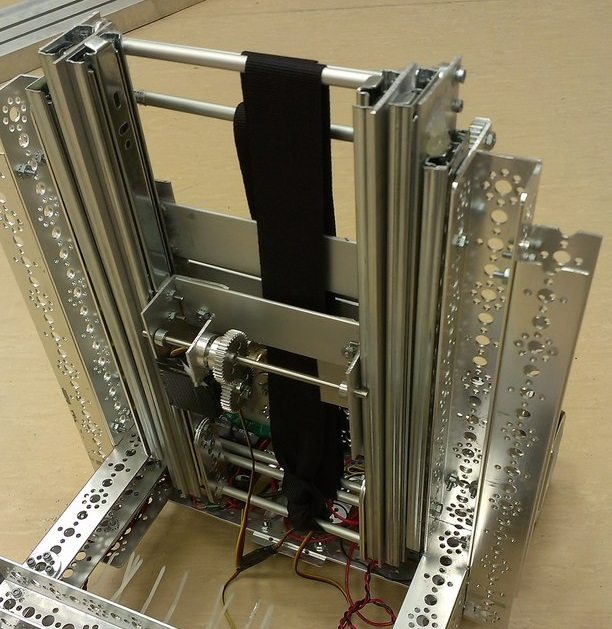
\includegraphics[scale=0.3]{days/01.11.14/images/01}}
      		\caption{Lift is finished}
      	\end{minipage}
      \end{figure}
      
      \item	Lift was tested by pulling the belt by hands. We found that extracting the lift demands some effort. 2 drives must cope with this task. Inner pair rails did not fall under their own weight during the lowering. We decided to increase their weight and reduce friction.
      
      \item	 Mechanism of extracting the lift was installed on the robot (hereinafter it will be called as MEL).
      
      \begin{figure}[H]
      	\begin{minipage}[h]{1\linewidth}
      		\center{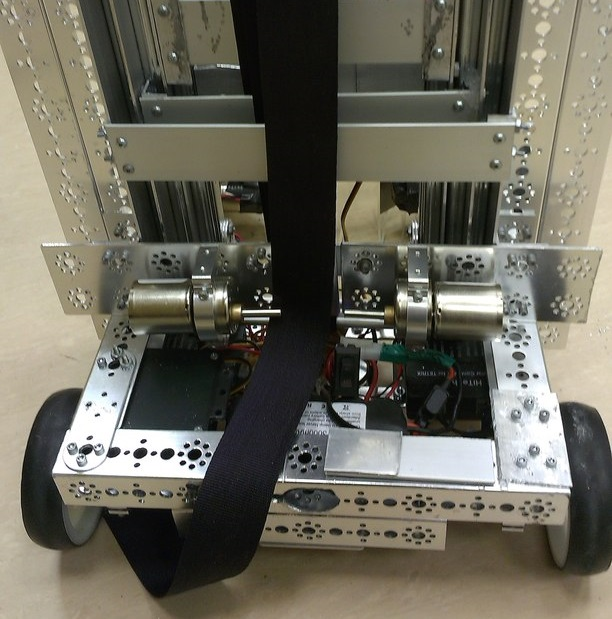
\includegraphics[scale=0.3]{days/01.11.14/images/02}}
      		\caption{Drives for moving lift}
      	\end{minipage}
      \end{figure}
      
    \end{enumerate}
    
	\item Results: 
	\begin{enumerate}
	  \item	The rib was installed.
	  
	  \item	MEL was done.
	  
	  \item	The lift was tested.
	  
	  \item	Installation of the MEL was started.
	   
    \end{enumerate}
    
	\item Tasks for the next meetings:
	\begin{enumerate}
	  \item	Finalize the mechanism winch.
	  
	  \item	Install the drivers for the winch.
	  
	  \item	Fix the belt with thread.
	  
	  \item	Replce NXT-brick.
	  
    \end{enumerate}     
\end{enumerate}
\fillpage
